\chapter{Interpretation of morphogen gradients by a synthetic bistable circuit}
\label{chapter:double-exclusive}
%\epigraph{``No person will deny that the highest degree of attainable accuracy is an object to be desired, and it is generally found that the last advances towards precision require a greater devotion of time, labour, and expense, than those which precede them."}{Charles Babbage}

\begin{enumerate}
    \item Keep focus on developmental biology
    \item Revised supplement as this chapter
\end{enumerate}

\usetikzlibrary{patterns}
\begin{Figure}
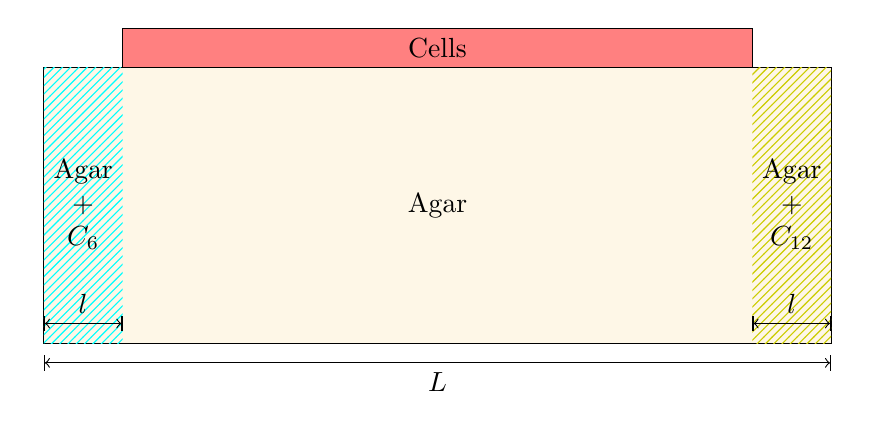
\begin{tikzpicture}
\def\H{3.5}
\def\L{10.0}
\def\l{1.0}
\def\epsilon{0.5}
\def\dx{0.25}
\def\dy{0.25}

%cell region
\filldraw[fill=Red!50!white] (\l,\H) rectangle (\L-\l,\H+\epsilon) node[midway] {Cells};

%agar region
\filldraw[fill=Dandelion!10!white,draw=black] (0,0) rectangle (\L,\H) node[midway] {Agar};
\fill[pattern=north east lines, pattern color=cyan] (0,0) rectangle (\l,\H) node[midway] {\begin{tabular}{c}Agar\\+\\$C_6$\end{tabular}};
\fill[pattern=north east lines, pattern color=yellow!80!black] (\L-\l,0) rectangle (\L,\H) node[midway] {\begin{tabular}{c}Agar\\+\\$C_{12}$\end{tabular}};
\draw[|<->|](0,-\dy) -- (\L,-\dy) node[midway, below] {$L$} ;
\draw[|<->|](0,\dy) -- (\l,\dy) node[midway, above] {$l$} ;
\draw[|<->|](\L-\l,\dy) -- (\L,\dy) node[midway, above] {$l$} ;
%\draw[|<->|](\L+\dx,0) -- (\L+\dx,\H) node[midway, right] {$H$} ;
%\draw[|<->|](\L+\dx,\H) -- (\L+\dx,\H+\epsilon) node[midway, right] {$H_\varepsilon$} ;

%axis
%\draw[->] (-\dx-\dy,-\dy)--(0.1*\L,-\dy) node[right] {$x$};
%\draw[->] (-\dx,-\dx-\dy)--(-\dx,0.5*\H) node[above] {$y$};
\end{tikzpicture}
\caption{Geometry of opposing gradients experiment}
\label{fig:experiment_geometry}
\end{Figure}

This section outlines how the Design---Learn pipeline may help achieve a specific
aim in a typical collaboration between theory, computation and experiment.
The aim of this project is to reconstitute and control minimal self-organisation
mechanisms which are believed play crucial roles in developmental biology. To this
end \textit{E. Coli} has been genetically engineered to produce orthogonal responses
to two different input signals --- henceforth this organism will be referred to as the
\textit{double exclusive reporter} circuit \cite{Grant2016}. The colony of reporters
serve as a reduced model for a multi-cellular organism during embryonic stages of
development. While patterns with sharp boundaries have successfully been realised,
producing Turing instabilities remains challenging as the system needs to be such
that patterns develop before the colony reaches stationary phase.
The role of theory and computation in this project is to help identify the
parameter regimes that produce controllable and self-organised patterns.

\section{Developmental Context}
During the development of any organism a hierarchy of self-organisation takes place that leads
to the breaking of symmetry from a spherical cluster of undifferentiated cells to the formation
of organ segments and limbs. This process is known as morphogenesis. figure \ref{fig:morph}
shows an example in which \textit{Hox} gene expression patterns in the body segments of
Drosophila can drastically affect its development.

\begin{Figure}
\includegraphics[width=90mm]{figures/morph1.png}\\
\includegraphics[width=90mm]{figures/morph2.png}
\caption{Top: \textit{Hox} gene expression patterns in body segments of drosophila.\\
Bottom: Mutation where legs grow in-place of antenna \cite{Urry2017CampbellBiology}}
\label{fig:morph}
\end{Figure}
\subsection{Morphogen-driven Patterns}
One of the central questions in developmental biology is how positional information is
sensed by a population of cells and how sharp gene expression boundaries between
populations are maintained for robust organ and body segment development. The
French Flag model \cite{Wolpert1969PositionalDifferentiation.} proposes that cells
have a threshold response to external signalling molecules -- henceforth referred
to as morphogens -- which pre-pattern the organism from anterior to posterior and
laterally. Some examples of morphogens include Wingless, Decapentaplegic and Sonic Hedgehog.
figure \ref{fig:gap} show the \textit{Gap} expression patterns that partition the
Drosophila embryo into segments which are later differentiated by \textit{Hox} genes.

\begin{Figure}
\includegraphics[width=90mm]{figures/gap.jpg}
\caption{Expression patterns of pair-rule \textit{Gap} genes in Drosophila embryo \cite{}}
\label{fig:gap}
\end{Figure}

\subsection{Self-organised Patterns}
How are morphogen gradients set up and maintained? How can they be robust against
changes in size and geometry? A canonical example of self-organisation in bacteria
is the quorum sensing system \cite{Miller2001QuorumBacteria}. Each cell secretes a
signalling molecule resulting in the total concentration being proportional to
the population density. This signal induces adaptive responses in metabolic and
mobility in the whole colony. A long standing mathematical hypothesis that
Turing patterns underlie self-organisation in cell populations. Recent literature
suggests both morphogen-driven and Turing patterning mechanisms play a role in development 
\cite{Green2015PositionalCombine}

\begin{Figure}
\includegraphics[width=70mm]{figures/turing.png}
\caption{Pigment patterns hypothesised to be generated by Turing mechanism}
\label{fig:gap}
\end{Figure}

\section{Methods and Results}
This section outlines the results on determining the bi-stability landscape for the
\textit{double-exclusive reporter}, and how its geometry helps determine the conditions for
moving and stationary sharp boundary formation. The design of the device is summarised 
in figure \ref{fig:device}. Each wiggly line represents a promoter. Incoming solid lines
to a vertex represents the formation of a complex, which lead to the induction of a promoter.
Outgoing solid lines represent the transcription-translation of genes downstream of a
promoter. Arrows that end in t-junctions represent the repression of a pathway.

\begin{Figure}
\includegraphics[width=140mm]{figures/device.png}
\caption{Left: Diagram of double exclusive reporter showing wiring between promoters
and complexes Right: Repression of \textit{pTet} and \textit{pLac} promoters via
\textit{TetR} and \textit{LacI} respectively}
\label{fig:device}
\end{Figure}
\noindent
The observable chemicals, labelled \textit{YFP} and \textit{CFP}, are
proportional to their upstream promoter activities. The experimentally controllable chemicals
are quorum sensing molecules $C_6$, $C_{12}$ and de-repressesors \textit{ATC},\textit{IPTG}.
All other chemicals cannot be directly observed. The double-negative feedback loop leads
to bi-stability in the observable signals, which is key to producing sharp gene
expression boundaries.

\begin{Figure}

\includegraphics[width=120mm]{figures/microtiter.png}
\includegraphics[width=100mm]{figures/parameter-space.png}
\caption{Top Left: Optical density measurements obtained for one well.
Top Right: Final fluorescence values at 16h across different $C_6$, $C_{12}$
concentrations. Bottom: Steady state predictions between data regions.}
\label{fig:data}
\end{Figure}

\subsection{Microtiter Plate Data}
The synthetic bacterial cultures are grown in suspended media and plated on
96 well microtiter plates in different concentrations of signalling molecules
$C_6$, $C_{12}$ and de-repressesors \textit{ATC},\textit{IPTG}. Then
optical density measurements in \textit{YFP} and \textit{CFP} are taken
from each well every 20min for 16 hours. Cells begin to grow in exponential
phase where the circuit is assumed to function optimally, until the
population eventually reaches stationary phase. figure \ref{fig:data} across
several different conditions overlayed on top of a model what predicts
the steady state behaviour between collected data regions.

\subsection{Spatial Experiments}
Simulations of the model revealed that if the final homogenous concentrations
of $C_6$ and $C_{12}$ lie within the bistable region, then the prepatterned
signals will form a sharp boundary at their interface. Spatial experiments
shown in figure \ref{fig:boundary} confirm this prediction.
\begin{Figure}
\includegraphics[width=120mm]{figures/spatial.png}
\caption{Merge channel yfp/cfp kymographs showing stationary (right)\\and moving boundaries (left)}
\label{fig:boundary}
\end{Figure}


Contributions for this work are as follows: \textbf{Mohamed Ali al-Badri} and \textbf{Christian D. Lorenz} conceived and planned the research. \textbf{Mohamed Ali al-Badri} and \textbf{Robert C. Sinclair} developed the nanomaterial structure software. \textbf{Mohamed Ali al-Badri} performed the calculations. \textbf{Mohamed Ali al-Badri, Paul Smith} and \textbf{Christian D. Lorenz} analysed the data and \textbf{Mohamed Ali al-Badri} prepared the final manuscript.

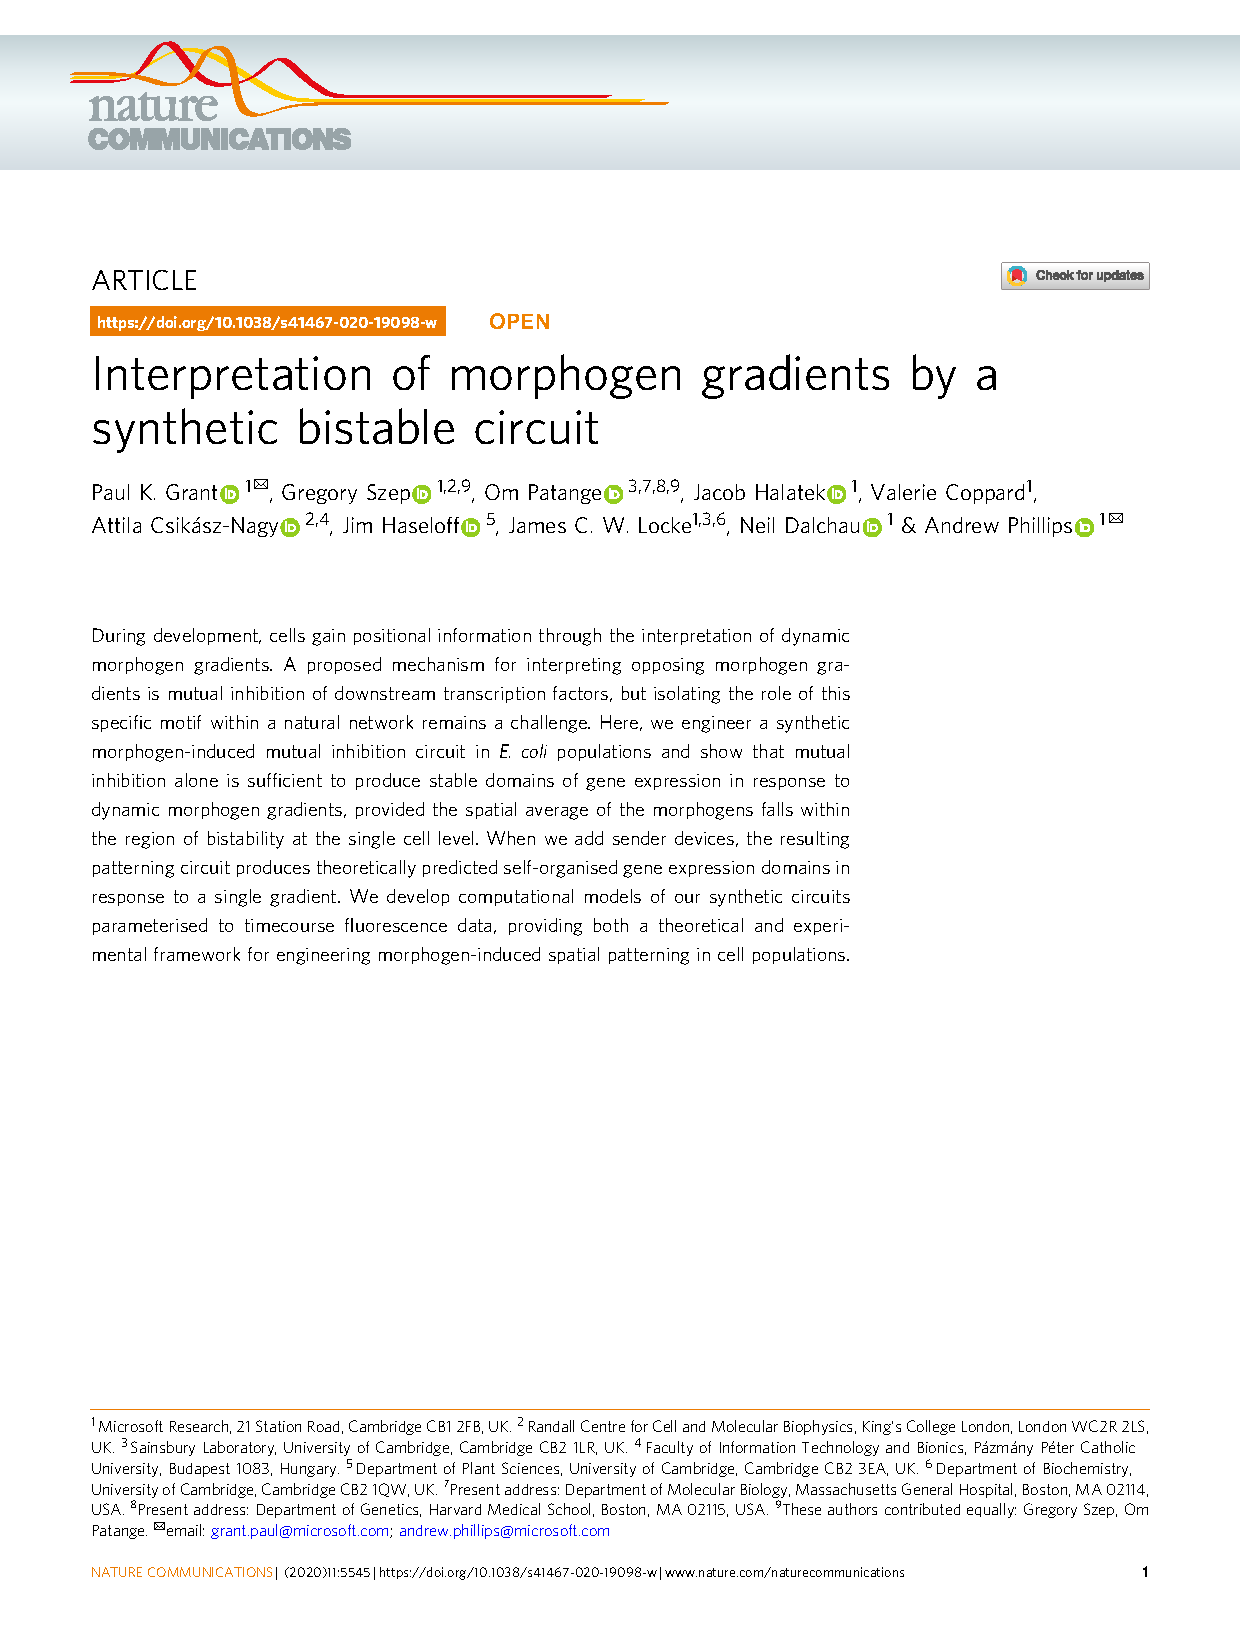
\includepdf[pages=-, offset=75 -75, addtotoc={
        2,section,1,Introduction,section:introduction,
        2,section,1,Results,section:results,
        2,subsection,2,Engineering mutual exclusivity,exclusivity,
        3,subsection,2,Mutual inhibition results in bistability,bistability,
        4,subsection,2,Hysteresis produces stable boundaries,boundaries,
        4,subsection,2,A secondary gradient creates self-organised domains,self-organisation,
        5,section,1,Discussion,section:discussion,
        6,section,1,Methods,section:methods,
        6,subsection,2,Plasmid construction,plasmids,
        6,subsection,2,Plate fluorometer assay,plates,
        6,subsection,2,Flow-cytometric analysis of hysteresis,flow,
        7,subsection,2,Microfluidics,microfluidics,
        7,subsection,2,Microfluidics microscopy,microscopy,
        7,subsection,2,Solid culture assays,cultures},
    addtolist={
        2, figure, {\textbf{A synthetic gene circuit for morphogen interpretation}. \textbf{a} Schematic representation of a developing embryo. Mutual inhibition of transcriptionfactors (cyan and yellow) downstream of antiparallel morphogen gradients (dark blue and orange) has been hypothesized to produce mutually exclusive domains of gene expression. \textbf{b} Morphogen gradients can be dynamic and transient, yet sharp, stable boundaries are observed between domains of gene expression. \textbf{c} A diagram of the Exclusive Receiver circuit. When 3O-C12-HSL (C12) levels are high, C12 binds to LasR, activating the expression of YFP and TetR, which represses the expression of LuxR, preventing expression of CFP and LacI. When 3O-C6-HSL (C6) levels are high, C6 binds to LuxR activating expression of CFP and LacI, which represses the expression of LasR, preventing expression of YFP and TetR. \textbf{d} Fluorescence output, measured in microplate fluorometer assays, of the Exclusive Receiver (top) and the Receiver (bottom) circuits represented as a ratio of CFP- (left) or YFP- (right) fluorescence to RFP fluorescence during exponential phase, cultured in the presence of the concentrations of C6 and C12 indicated. Data are representative of $n=3$ biological replicate experiments conducted on different days}, figure:overview,
        3, figure, {\textbf{Mutual inhibition produces bistability}. Cells transformed with the Exclusive Receiver circuit were conditioned in either 500 nM C6 \textbf{a}, or 500 nM C12 \textbf{b}, and then exposed to the combinations of concentrations of C6 and C12 indicated.  Cells were measured using flow cytometry and their normalized CFP minus YFP expressions were plotted. The region of bistability predicted by the parameterized model is the area within the red lines.  \textbf{c}, Microfluidics cultures of cells transformed with Exclusive Receiver circuit in changing combinations of signals.  Cells were grown for 3 hours in the presence of either 37 nM C6 (rows 1 and 2) or 100 nM C12 (rows 3 and 4). Then media was changed to 100 nM C12 + 37 nM C6 (rows 1 and 3) or 100 nM C12 (row 2) or 37 nM C6 (row 4) . Cells were imaged with a frame rate of (1 frame/10 minutes). Left panels are kymographs of the log-ratio of CFP expression per-cell to YFP expression per-cell, and fraction of cells as a heat map.  Histograms represent the populations at 3 hours (red) and 8 hours (blue).  Lines and shaded region represent the mean and standard deviation, respectively, over {n = 4  biological replicates performed on 4 different days.} Right panels are sample montages of cells switching state (rows 2 and 4) or exhibiting bistablity (rows 1 and 3); phase contrast and fluorescence channel ranges chosen for display. Scalebar=6$\mu$m.}, figure:bistability,
        5, figure, {\textbf{Formation of stable boundaries.} \textbf{a}, Endpoint fluorescence microscopy of Exclusive Receiver cells grown in transient gradients of signals (C12 diffusing from the left, C6 diffusing from the right) at the spatial average concentrations indicated and in the context of 10 $\mu$M IPTG throughout.  Representative examples (n=3 biological replicates performed on 3 different days) of a static boundary (left) and a moving boundary (right) \textbf{b}, Corresponding kymographs of CFP and YFP fluorescence (intensity) over time (y-axes, hours) at different spatial positions (x-axes, mm). If the location of the boundary (location of equal normalized CFP and YFP fluorescences, black lines) at the end of the timelapse minus its location when it became detectable ($\Delta\beta$, arrows) was less than 10\% of the domain size we considered the boundary stable.   \textbf{c}, Boundaries were evaluated as above at the signal concentrations indicated by letters. ‘S’ indicates equilibrium concentrations at which static boundaries were observed. ‘M’ indicates a moving boundary. 'N' indicates no boundary.  The color of the letter indicates which FP was dominant and red indicates neither FP dominant. \textbf{d}, Schematic representation of the concentrations of C6 and C12 experienced by cells at different points in physical space (cyan and yellow curves) as gradients diffuse to homogeneity.  Paler curves represent different timepoints.  If the spatial average concentrations lie within the region of bistability, the boundary will be static (S), otherwise the boundary will move (M) and will eventually be abolished as cells adopt either CFP or YFP expression.   $t_1$ and $t_2$ indicate timepoints considered in (e).  \textbf{e}, Corresponding schematic representing LasR expression, colored according to resultant fluorescent protein expression.  Dashed line indicates the location of an unstable local equilibrium. Red lines indicate the spatial location in which cells are exhibiting bistability.  In the case of a stationary boundary (S), the region of space containing cells exhibiting bistability expands to encompass all cells and their gene expression state is determined by their history.  In the case of a moving boundary (M), the region exhibiting bistability moves rightward and disappears and the domain becomes dominated by a single monostable state.}, figure:boundaries,
        6, figure, {\textbf{Addition of a Relay circuit creates self-organised domains of gene expression.} \textbf{a}, Circuit diagram of Exclusive Receiver cells co-transformed with a  Relay circuit  (P76-LasI) that responds to C6 by producing C12. \textbf{b}, Isogenic cells transformed with the circuit shown in (a) and grown for 24 hours in the presence of a gradient of C6 diffusing from the centre. Cells that experience high levels of C6 (central cells) will express CFP, LacI, and LasI, causing them to produce C12 but be unable to sense it.  Neighbouring cells (outer cells) that do not experience C6 will sense C12 and express YFP and TetR, resulting in mutually exclusive domains of gene expression.{ Cells also constitutively express mRFP1 via a genomic transgene. Image is representative of 3 biological replicates performed on 3 different days.} \textbf{c}, Quantitation of fluorescence along the dotted line in b. Cyan, yellow, and red indicate CFP, YFP, and RFP expression, respectively. \textbf{d}, Final timepoint of simulation shows a secondary gradient of C12 (orange) produced in response to the primary C6 gradient (dark blue).  Cyan and yellow indicate simulated CFP and YFP expression, respectively.  \textbf{e}, Final time point of simulation in C6-C12 space labelling points in physical space by their CFP and YFP expression (cyan and yellow points), and showing the production of C12 as vectors (red arrows) that move the spatial average (x) toward increasing C12}, figure:relay
}]{publications/double-exclusive.pdf}